\part{Metodologia}

\chapter[Metodologia]{Metodologia}

Este capítulo é destinado à apresentar toda a metodologia aplicada a esta
pesquisa. Vale ressaltar que a metodologia proposta nesta pesquisa está sendo
baseada na definição proposta por Silva e Menezes, que afirmam que toda pesquisa
tem como objetivo encontrar respostas para hipóteses propostas
\cite{da2005metodologia}

Com essa definição em pauta, as hipóteses proposta para a execução deste trabalho neste trabalho foi a seguinte:

\begin{center}
\textit{É possível melhorar a recomendação baseada em conteúdo de pacotes para
usuários de sistemas GNU/Linux levando em consideração o contexto de uso dos pacotes já instalados ?}
\end{center}

Baseado nesta hipótese central, pode-se ver que a pesquisa sendo desevolvida se
enquadra como aplicada, quantitativa, exploratória, bibliográfica e
experimental.


\section{Trabalhos relacionados}

Durante a pesquisa deste trabalho, encontrou-se alguns trabalhos que também estudam recomendação baseada em contexto, sendo o tempo um dos
principais atributos do contexto. Em \cite{lee2008time}, o tempo é usado para gerar avaliação implícita para um histórico de
compras de diversor usuários. Tal abordagem foi comparada com um modelo de recomendação colaborativa tradicional, usando avaliação explícita dos usuários,
sem considerar o tempo. Segundo a pesquisa, percebeu-se um aumento de precisão quando o tempo foi usado para gerar a matriz de recomendação.

Outra pesquida relacionada foi a de \cite{ding2005time}. Nesta pesquisa, um sistema recomendação sensível ao tempo foi criado. o sistema proposto usava uma função de
decaimento exponencial para priorizar itens recentemente avaliados e diminuir o peso de itens avaliados a mais tempo na recomendação. Quando comparado a um sistema de
recomendação colaborativa clássico, percebeu-se um aumento de acurácia para o recomendador sensível ao tempo.

Além de comparação de sistema de recomendação, foi também encontrado um trabalho que propõe um modelo diferente do clássico uso do tempo em recomendação, como o usado em
\cite{ding2005time}. Este modelo foi proposto no artigo de \cite{basile2015modeling}, onde basicamente itens mais antigos não tem seu peso puramente discartado, e sim caso
seu conteúdo seja diferente dos novos itens sendo recomendados. Baseado nos testes realizados, percebeu-se que criar o modelo de usuário dessa formas apresenta vantagens sobre
a forma mais padrão de se usar o tempo para recomendação. Entretanto, o trabalho ainda precisa ser testado em bancos de dados de maior escala para poder aferir melhor seus
resultados

Por fim, um famoso trabalho que usa o contexto de tempo para recomendação se dá na pesquisa \cite{koren2010collaborative}, que apresenta o modelo de recomendação vencedor
do concurso criado pelo Netflix para aumentar a acurácia de suas recomendações de filme. A pesquisa citada usa como diferencial a análise do tempo da avaliação dos filmes
realizados pelos usuários em um modelo similar a pesquisa de \cite{basile2015modeling}
    

\section{Hipóteses}

Considerando um sistema de recomendação para pacotes usando o tempo como variável de contexto, as seguinte hipóteses foram definidas:

\begin{itemize} \item \textit{\textbf{Ao aumentar o peso de pacotes
recentemente usados no sistema, o perfil do usuário gerado será mais preciso,
ocasionando assim uma recomendação mais apropriada.}} Considerando que o perfil
do usuário na recomendação é gerado pelo termos encontrados em maior presença
em todos os pacotes manualmente instalados pelo usuário, é uma possibilidade
aumentar o peso dos termos de pacotes recentemente usados e diminuir o peso de
pacotes antigos, irá gerar um perfil que melhor espelha as prioridades do
usuário, gerando assim uma recomendação de maior precisão \item
\textit{\textbf{Uma abordagem determinística para o problema irá se comportar
pior que uma não-determinística quando se usa o tempo de uso como contexto de
classificação}} Uma abordagem deterministica iria modificar o atual perfil do
usuário usado para gerar a recomendação sendo gerada, entretanto uma abordagem
não deterministica, baseada no aprendizado de máquina, irá refinar as
recomendações geradas usando a configuração atual. Considerando a complexidade
dos dados presentes em um pacote Debian, juntamente com os relacionamentos
entre tais atributos, acredita-se que uma abordagem não-deterministica irá
prover melhores resultados. 
\end{itemize}

\section{Planejamento da pesquisa}

Com o intuito de responder a questão principal do trabalho, juntamente com as
hipóteses propostas, um fluxo de trabalho foi definido. A Figura
\ref{fig:planejamento_pesquisa} sistematiza tal fluxo, facilitando assim a visualização do processo adotado.

\begin{figure}[h]
  \centering
  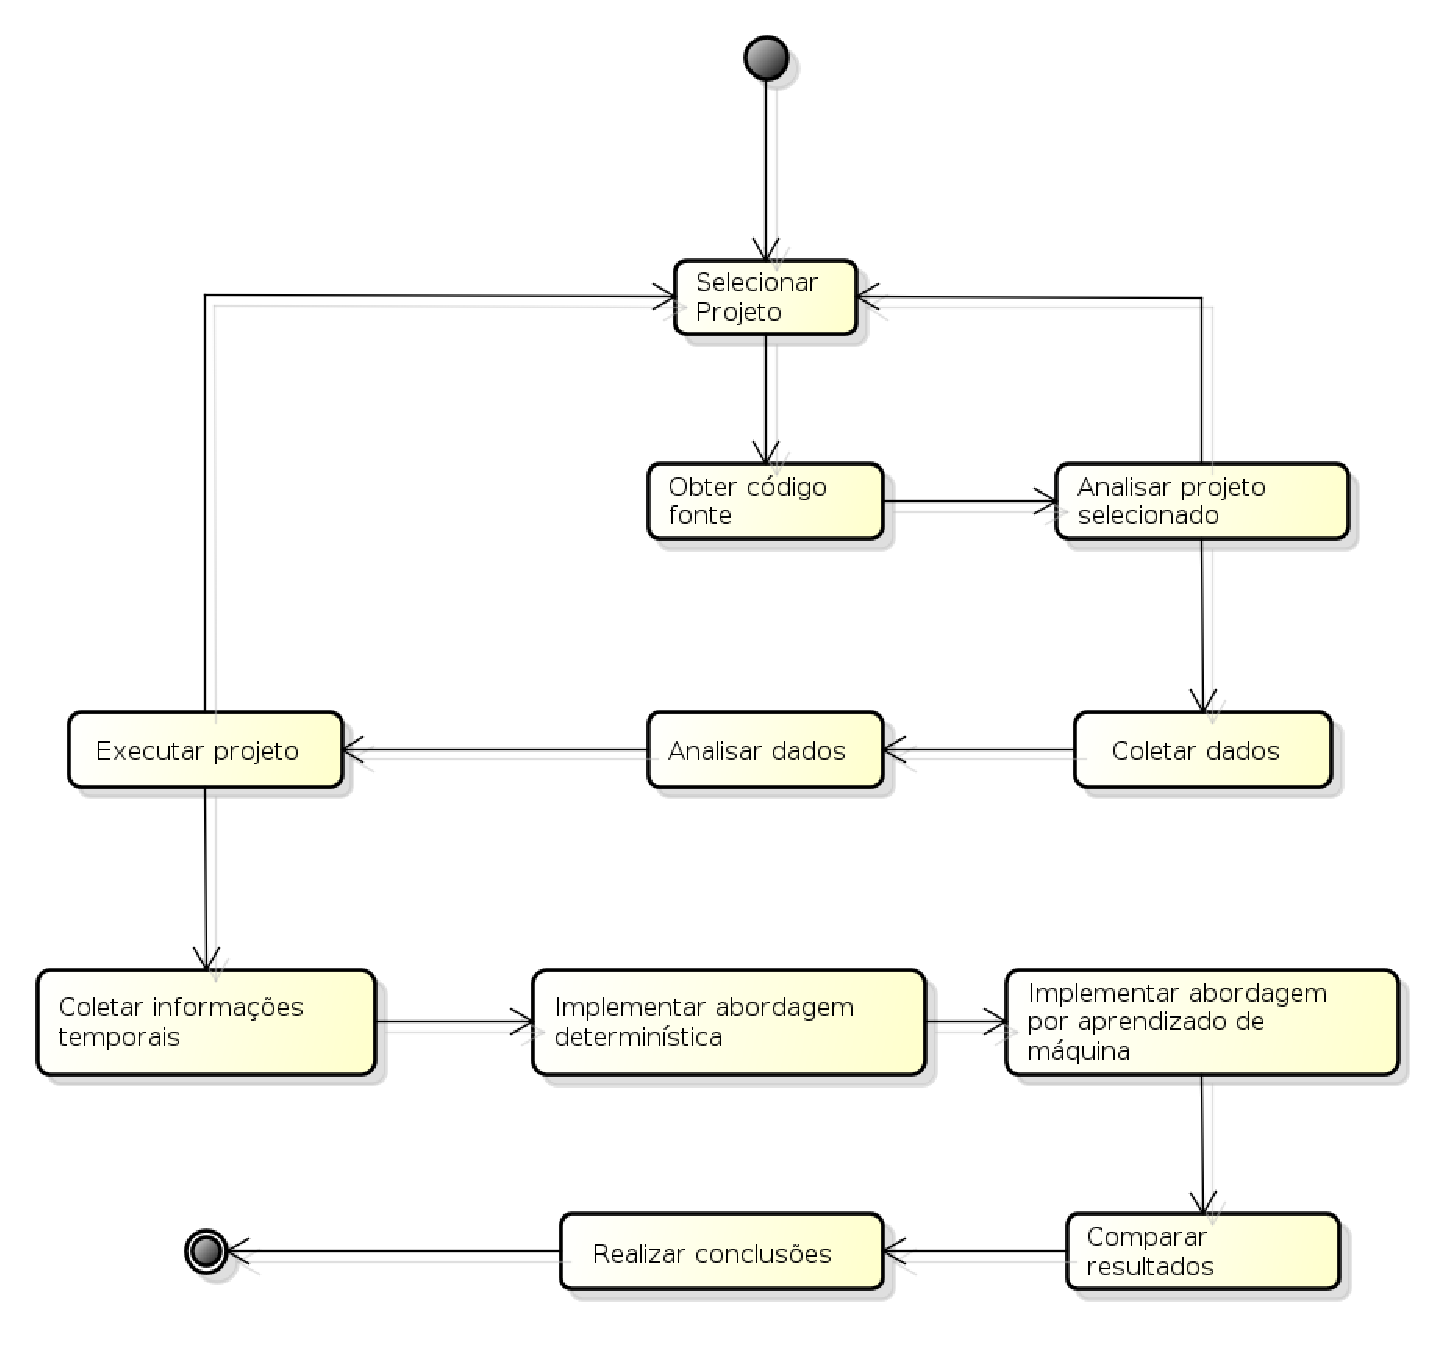
\includegraphics[width=0.9\textwidth]{figuras/planejamento_pesquisa.eps}
  \caption{Processo usando para realização das atividades dessa pesquisa}
  \label{fig:planejamento_pesquisa}
\end{figure}

\begin{enumerate}

    \item \textbf{Selecionar projeto:}
Selecionar um projeto de software livre que implemente um sistema de recomendação baseada em conteúdo e que não leve em consideração questões temporais do pacote quando se realiza tanto
a criação do perfil de usuário e a recomendação propriamente dita. Além disso, deve-se também levar em consideração as dependências do projeto, desde os bibliotecas que depende e os
dados necessitados. Caso o projeto necessite de dados que não possam ser obtidos pelo pesquisadores deste trabalho, o mesmo não poderá ser considerado.

    \item \textbf{Obter código fonte:}
Obter o código fonte do projeto em questão, para que o mesmo possa ser alterado visando o estudo das hipóteses levantadas

    \item \textbf{Analisar projeto selecionado:}
Nesta etapa, o projeto deve ser analisado, visando a compreensão de como o mesmo funciona e, principalmente, os dados necessários para a execução adequada do projeto.

    \item \textbf{Coletar dados:}
Para prover os possíveis dados necessários para o projeto selecionado, uma estratégia de coleta de dados precisa ser definida e implementada.

    \item \textbf{Análisar dados:}
Será necessário analisar os dados coletados, visando descartar dados inválidos e classificar o que foi coletado conforme as necessidades do projeto escolhido.

    \item \textbf{Executar projeto selecionado:}
Com os dados e as dependências do projeto resolvidas, o mesmo deve ser executado, visando encontrar possíveis problemas de execução que não foram previstos e também observar as funcionalidades do projeto.

    \item \textbf{Coletar informações temporais:}
Deve-se implementar uma forma de coletar as informações temporais dos pacotes sendo usados pelo usuário e também prover uma forma de classificar essa informação coletada.

    \item \textbf{Implementar abordagem deterministica:}
Para responder a primeira questão proposta, será necessária implementar uma equação matemática que use as informações de tempo coletadas, juntamente com os outros atributos já usados no projeto selecionado para prover um recomendação.

    \item \textbf{Implementar abordagem por aprendizado de máquina:}
Implementar uma abordagem não-deterministica, no caso uma estratégia de aprendizado de máquina, para usar as informações de tempo coletadas juntamente com os outros atributos providos pelo projeto selecionado para compor um a recomendação.

    \item \textbf{Comparar resultados:}
Para responder as hipóteses propostas será necessário não só comporar as duas abordagens propostas, determinística e não determinística, e sim comparar ambas também com as abordagens já implementadas pelo projeto proposto e verificar se as hipótes se sustetam.

    \item \textbf{Realizar conclusões:}
Com a comparações de resultados feita, a mesma deve ser analisada e conclusões devem ser geradas baseada nos fatos apresentados.
\end{enumerate}


\section{Teste de hipótese}

O projeto selecionado para testar as hipóteses foi o \textit{AppRecommender}, o recomendador de pacotes para distribuições Debian que implementa tanto estratégias de recomendação por conteúdo quanto colaborativas \cite{araujo2011apprecommender}. 
Apesar do AppRecommender usar questões temporarais providas pelo pacote popularity-contest nas suas recomendações, tal atributo temporal só é explorado nas recomendações colaborativas, e não nas baseadas em conteúdo, fazendo com que o projeto passe no critério de seleção estabelecido.

\begin{description}

\item[Obtenção do código fonte]

O código fonte da aplicação AppRecommender pode ser encontrada no repositório de projetos Github \footnote{\url{https://github.com/tassia/AppRecommender}}.
Vale ressaltar que as modificações realizadas foram realizadas em uma cópia local do mesmo, sendo essa mantida pelos pesquisadores deste trabalho.

\item[Analisar projeto selecionado]

Um vez obtido o código fonte do projeto, identificou-se algumas questõs
importantes. A primeira delas foi que algumas bibliotecas não estavam mais
presentes no repositório de pacotes de versões mais recentes do Debian, no caso,
o Debian jessie. A segunda problemática foi relacionada a obtenção do dados.
Mediante uma análise tanto do ponto de vista de recomendação tanto do ponto de
vista dos experimentos de validação usados para avaliar os algoritmos
desenvolvidos, percebeu-se diversos e distintos conjuntos de dados necessários.
A Tabela \ref{tab:dados_apprecommender} mostra os dados necessários e o contexto
onde são usados:
\end{description}

\begin{table}[h]
\centering
\resizebox{\textwidth}{!}{\begin{tabular}{|l|l|l|l|}
\hline
\rowcolor[HTML]{EFEFEF} 
{\textbf{Dados}} & {\textbf{Contexto}} & {\textbf{Coleta}} \\ \hline
Lista de pacotes válidos &
\parbox{10cm}{Esta lista irá ser usada na criação de uma índice de busca Xapian,
que será usado para realizar a recomendação} &
\parbox{10cm}{Pode-se usar os scripts get\_axipkgs.py obter todos os possíveis
pacotes Debian,ou usar o srcipt get\_programs.sh, que irá selecionar 
só pacotes que contém a Debtag role:;program, indicando que o mesmo é um
pacote executável.}\\ \hline
Índice xapian de pacotes do usuário &
\parbox{10cm}{Usado tanto para estratégias de recomendação por conteúdo,
 colaborativas e híbridas}&
\parbox{10cm}{Este Índice pode ser gerado via execução do script indexer\_axi.py
 passando os parâmetros certos}\\ \hline
Debtags válidas&
\parbox{10cm}{Usado para filtrar os pacote que serão usados na 
recomendação}&
\parbox{10cm}{Pode ser obtido pelo script get\_tags.py}\\ \hline
Submissões do popularity contest&
\parbox{10cm}{Usada para criar um índice Xapian de submissões do 
popularity-contest}&
\parbox{10cm}{O projeto não provê uma forma automatizada de coletar tais dados,
devido ao fato do mantenedor do projeto não fornecer tais dados.}\\ \hline
Indíce Xapian para submissões do popularity contest &
\parbox{10cm}{Usado tanto para a realização de recomendações colaborativas e 
híbridas, assim como para a execução dos experimentos usados 
para avaliar as soluções desenvolvidas.} &
\parbox{10cm}{Pode ser obtido pela execução do script indexer\_popcon.py.
Entretanto, vale ressaltar que esse script parte do princípio que já existem
submissões do popularity contest coletadas previamente.}\\ \hline
\end{tabular}}
\caption{Dados necessários para execução do AppRecommender}
\label{tab:dados_apprecommender}
\end{table}

Conforme pode ser observado na Tabela \ref{tab:dados_apprecommender}, muito dos dados
necessários para a execução do AppRecommender podem ser obtidos de forma automatizada
por scripts de coleta. Entretanto, este não é o caso para as submissões do
popularity contest. Isso se dá pelo fato da aplicação não disponibilizar as submissões
propriamente ditas, e sim as análises estatísticas feitas em cima das mesmas. Para o
AppRecommender, tais dados foram obtidos por intermédio de um Debian Developer, sendo
que algumas questões de relacionada a privacidade dos usuários se tornou necessária.
\cite{araujo2011apprecommender}. Dessa forma, foi necessário pensar em uma estratégia
de coleta de dados, principalmente visando o funcionamento dos experimentos propostos
para a avaliação dos algoritmos.

\subsection{Numeração de Páginas}

A contagem sequencial para a numeração de páginas começa a partir da 
primeira folha do trabalho que é a Folha de Rosto, contudo a numeração em 
si só deve ser iniciada a partir da primeira folha dos elementos textuais. 
Assim, as páginas dos elementos pré-textuais contam, mas não são numeradas 
e os números de página aparecem a partir da primeira folha dos elementos 
textuais que é a Introdução. 

Os números devem estar em algarismos arábicos (fonte Times ou Arial 10) no 
canto superior direito da folha, a 02 cm da borda superior, sem traços, 
pontos ou parênteses. 

A paginação de Apêndices e Anexos deve ser contínua, dando seguimento ao 
texto principal.

\subsection{Espaços e alinhamento}

Para a monografia de TCC 01 e 02 o espaço entrelinhas do corpo do texto 
deve ser de 1,5 cm, exceto RESUMO, CITAÇÔES de mais de três linhas, NOTAS 
de rodapé, LEGENDAS e REFERÊNCIAS que devem possuir espaçamento simples. 
Ainda, ao se iniciar a primeira linha de cada novo parágrafo se deve 
tabular a distância de 1,25 cm da margem esquerda.

Quanto aos títulos das seções primárias da monografia, estes devem começar 
na parte superior da folha e separados do texto que o sucede, por um espaço 
de 1,5 cm entrelinhas, assim como os títulos das seções secundárias, 
terciárias. 

A formatação de alinhamento deve ser justificado, de modo que o texto fique 
alinhado uniformemente ao longo das margens esquerda e direita, exceto para 
CITAÇÕES de mais de três linhas que devem ser alinhadas a 04 cm da margem 
esquerda e REFERÊNCIAS que são alinhadas somente à margem esquerda do texto 
diferenciando cada referência.

\subsection{Quebra de Capítulos e Aproveitamento de Páginas}

Cada seção ou capítulo deverá começar numa nova pagina (recomenda-se que 
para texto muito longos o autor divida seu documento em mais de um arquivo 
eletrônico). 

Caso a última pagina de um capitulo tenha apenas um número reduzido de 
linhas (digamos 2 ou 3), verificar a possibilidade de modificar o texto 
(sem prejuízo do conteúdo e obedecendo as normas aqui colocadas) para 
evitar a ocorrência de uma página pouco aproveitada.

Ainda com respeito ao preenchimento das páginas, este deve ser otimizado, 
evitando-se espaços vazios desnecessários. 

Caso as dimensões de uma figura ou tabela impeçam que a mesma seja 
posicionada ao final de uma página, o deslocamento para a página seguinte 
não deve acarretar um vazio na pagina anterior. Para evitar tal ocorrência, 
deve-se re-posicionar os blocos de texto para o preenchimento de vazios. 

Tabelas e figuras devem, sempre que possível, utilizar o espaço disponível 
da página evitando-se a \lq\lq quebra\rq\rq\ da figura ou tabela. 

\section{Cópias}

Nas versões do relatório para revisão da Banca Examinadora em TCC1 e TCC2, 
o aluno deve apresentar na Secretaria da FGA, uma cópia para cada membro da 
Banca Examinadora.

Após a aprovação em TCC2, o aluno deverá obrigatoriamente apresentar a 
versão final de seu trabalho à Secretaria da FGA na seguinte forma:

\begin{description}
	\item 01 cópia encadernada para arquivo na FGA;
	\item 01 cópia não encadernada (folhas avulsas) para arquivo na FGA;
	\item 01 cópia em CD de todos os arquivos empregados no trabalho;
\end{description}

A cópia em CD deve conter, além do texto, todos os arquivos dos quais se 
originaram os gráficos (excel, etc.) e figuras (jpg, bmp, gif, etc.) 
contidos no trabalho. Caso o trabalho tenha gerado códigos fontes e 
arquivos para aplicações especificas (programas em Fortran, C, Matlab, 
etc.) estes deverão também ser gravados em CD. 

O autor deverá certificar a não ocorrência de “vírus” no CD entregue a 
secretaria. 

